\documentclass[../sotsu.tex]{subfiles}

\graphicspath{{../fig/}}

\begin{document}

\section{ベクトル空間}
\label{sec:vector-space}

量子力学において,系の状態は「ベクトル」を用いてであらわされる.
しかし,通常の\ruby{数}{すう}ベクトルでは量子力学的状態をあらわせないことがわかる(ここでどこかを引用する).
そこで,数ベクトルの概念を一般化・抽象化する必要がある.
この章ではベクトルの性質を抽象化し,ベクトル空間について定義する.


\subsection{3次元ユークリッド空間$ℝ^3$の性質}

この節では,ユークリッド空間$ℝ^3$における数ベクトルの性質を確かめる.

$n$個の数字\footnote{ここでは実数または複素数のこと.}を縦に並べたものを「$n$-\ruby{次}{じ}の\ruby{列}{れつ}ベクトル」と呼び,
横に並べたものを「$n$-次の\ruby{行}{ぎょう}ベクトル」と呼ぶ\cite{miyake-lin-2008}.
列ベクトルのことを「\ruby{縦}{たて}ベクトル」,行ベクトルを「\ruby{横}{よこ}ベクトル」ということもある.

たとえば\cref{eq:complex-Euclidean-vector-example}の$𝒙$は3次の列ベクトル,
$𝒚$は3次の行ベクトルである.
\begin{align}
    \label{eq:complex-Euclidean-vector-example}
    𝒙 = 
    \begin{pmatrix}
        a  \\  b  \\  c
    \end{pmatrix}
    , \qquad
    𝒚 = 
    \begin{pmatrix}
        a  &  b  &  c
    \end{pmatrix}
    \qquad 
    \text{where $a, b, c ∈ ℂ$}
\end{align}
ここで,$a, b, c$はそれぞれある複素数である\footnote{$ℂ$は複素数全体の集合.\cref{eq:number-sets}を参照}.
$a, b, c$のことをそれぞれ,ベクトルの\word{成分}[せい|ぶん]という.

列ベクトルと行ベクトルは,「\word{転置}[てん|ち](transpose)」という操作によって移り変わる.
つまり,
\begin{equation*}
    \tp{\begin{pmatrix}
        a  \\  b  \\  c
    \end{pmatrix}}
    =
    \begin{pmatrix}
        a  &  b  &  c
    \end{pmatrix},
    \quad
    \tp{\begin{pmatrix}
        a  &  b  &  c
    \end{pmatrix}}
    =
    \begin{pmatrix}
        a  \\  b  \\  c
    \end{pmatrix}
\end{equation*}
である.
列ベクトルを,転置を用いて$\tp{(a \quad b \quad c)}$と表記することもある.

ベクトル$\tp{(a, b, c)}$は,ある点から$x$-軸方向へ$a$,$y$-軸方向へ$b$,$z$-軸方向へ$c$だけ動いた点を結ぶ矢印として考えることができる.


\subsubsection*{ベクトルの演算}

ベクトル同士の「\ruby{和}{わ}」(足し算)を
\begin{equation*}
    \begin{pmatrix}
        a  \\  b  \\  c
    \end{pmatrix}
    \vecplus
    \begin{pmatrix}
        a' \\ b' \\ c'
    \end{pmatrix}
    =
    \begin{pmatrix}
        a + a'  \\  b + b'  \\  c + c'
    \end{pmatrix}
\end{equation*}
のように,各成分の和として定義する.
ベクトルの和は,2つの矢印をつなげた見たときの矢印に相当する(\cref{fig:vector-sum}).

また,ベクトルの「スカラー倍」を,
\begin{equation*}
    𝜆 \scaprod 
    \begin{pmatrix}
        a  \\  b  \\  c
    \end{pmatrix}
    =
    \begin{pmatrix}
        𝜆 a  \\  𝜆 b  \\  𝜆 c
    \end{pmatrix}
\end{equation*}
で定義する.
ベクトルのスカラー倍は,向きを保ったまま長さを$𝜆$倍した矢印に対応する(\cref{fig:vector-scalar-p}).

\begin{figure}[tbp]
    \centering
    \begin{subcaptionblock}{0.4\linewidth}
        \centering
        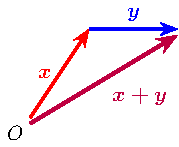
\includegraphics[width=0.9\linewidth]{vector_sum.pdf}
        \caption{ベクトルの和}
        \label{fig:vector-sum}
    \end{subcaptionblock}
    \begin{subcaptionblock}{0.4\linewidth}
        \centering
        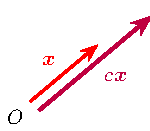
\includegraphics[width=0.9\linewidth]{vector_scalar_p.pdf}
        \caption{ベクトルのスカラー倍}
        \label{fig:vector-scalar-p}
    \end{subcaptionblock}
    \caption{ベクトルの演算}
\end{figure}


\subsubsection*{ベクトルの内積}

$\symbf{a}$と$𝒙$を列ベクトルとすると,
それらの間の\refdfn[内積]{dfn:inner-product}は,以下のように定義できるのだった.
\begin{equation*}
    (\symbf{a}, 𝒙)
        = \symbf{a} \cdotp 𝒙
        = \norm{\symbf{a}} \norm{𝒙} \cos \theta
\end{equation*}
ここで,$\norm{\symbf{a}}$はベクトル$\symbf{a}$の\refdfn[長さ]{dfn:norm}であり,
これは三平方の定理より
\[  \norm{\symbf{a}} = \sqrt{ a^2 + b^2 + c^2 }  \]
で与えられる.
また,$\theta$は$\norm{\symbf{a}}$と$\norm{𝒙}$のなす角度である.

2つのベクトルが\refdfn[直交]{dfn:orthogonal}する場合($\theta = \pi/2$),
$\cos \theta = 0$となるから,内積は$0$になる.



\subsection{ベクトル空間の定義}

\begin{definition}[ベクトル空間]
    \label{dfn:vector-space}
    $V$を集合,$(𝕂, +, \dotprod)$を体\refdfn{dfn:field}とする.
    $V$上の\word{和}$\vecplus\colon V \times V \to V$,\word{スカラー倍}$\scaprod \colon 𝕂 \times V \to V$が定義され,
    以下が満たされるとき,$(V, \vecplus, \scaprod)$を($𝕂$上の)\word{ベクトル空間}(vector space)あるいは\word{線形空間}[せん|けい|くう|かん](linear space)という.
    このとき$V$の元を\word{ベクトル}(vector),$𝕂$の元を\word{スカラー}(scalar)という.
    \begin{enumerate}
        \item \label{vector:sum-associative} 任意の$𝒖, 𝒗, 𝒘 ∈ V$に対して,$(𝒖 \vecplus 𝒗) \vecplus 𝒘 = 𝒖 \vecplus (𝒗 \vecplus 𝒘)$である.
        \item \label{vector:sum-zero} ある$\symbf{0} ∈ V$がただひとつ存在し,任意の$𝒗 ∈ V$に対して,$𝒗 \vecplus \symbf{0} = \symbf{0} \vecplus 𝒗 = 𝒗$である.
        \item \label{vector:sum-opposite} 任意の$𝒗 ∈ V$に対して,ある$-𝒗$がただひとつ存在して,$𝒗 \vecplus (-𝒗) = (-𝒗) \vecplus 𝒗 = \symbf{0}$である.
        \item \label{vector:sum-commutative} 任意の$𝒖, 𝒗 ∈ V$に対して,$𝒖 \vecplus 𝒗 = 𝒗 \vecplus 𝒖$である.
        \item \label{vector:scalar-distributive} 任意の$𝒖, 𝒗 ∈ V$および任意の$c ∈ 𝕂$に対して,$c \scaprod (𝒖 \vecplus 𝒗) = (c \scaprod 𝒖) \vecplus (c \scaprod 𝒗)$である.
        \item \label{vector:scalar-sum} 任意の$𝒗 ∈ V$および任意の$a, b$に対して,$(a + b) \scaprod 𝒗 = (a \scaprod 𝒗) \vecplus (b \scaprod 𝒗)$である.
        \item \label{vector:scalar-prod} 任意の$𝒗 ∈ V$および任意の$a, b$に対して,$(a \dotprod b) \scaprod 𝒗 = a \scaprod (b \scaprod 𝒗)$である.
        \item \label{vector:scalar-identity} 任意の$𝒗 ∈ V$に対して,$1 \scaprod 𝒗 = 𝒗$である.
    \end{enumerate}
    ベクトル空間$(V, \vecplus, \scaprod)$のことを単に$V$と書くこともある.
\end{definition}

\cref{dfn:vector-space}は,
ユークリッド空間における数ベクトルがもつ性質を抽出したものである.

\begin{corollary}
    ベクトル空間$V$は以下を満たす.
    \begin{itemize}
        \item 任意の$𝒗 ∈ V$に対し,
        \begin{enumerate}[resume]
            \item $ 0 \scaprod 𝒗 = \symbf{0} $である.
            \item $ (-1) \scaprod 𝒗 = -𝒗 $である.
        \end{enumerate}
    \end{itemize}
\end{corollary}

\begin{proof}
    \begin{enumerate}
        \item $ 0 \scaprod 𝒗 = (0 + 0) \scaprod 𝒗 = 0 \scaprod 𝒗 \vecplus 0 \scaprod 𝒗 $より従う.
        \item $ 𝒗 \vecplus (-1) \scaprod 𝒗 = 1 \scaprod 𝒗 \vecplus (-1) \scaprod 𝒗 = (1 + (-1)) \scaprod 𝒗 = 0 \scaprod 𝒗 = \symbf{0} $より従う.
    \end{enumerate}
\end{proof}

$𝒗 \vecplus (-𝒖) \eqcolon 𝒗 \vecminus 𝒖$とかくことが多い.



\subsection{部分ベクトル空間}

\begin{definition}[部分ベクトル空間]
    \label{dfn:vector-subspace}
    $V$をベクトル空間,$W \subset V$とする.
    $W$が$V$の和とスカラー倍に対してベクトル空間になるとき,$W$は$U$の\word{部分ベクトル空間}(vector subspace)あるいは単に\word{部分空間}(subspace)であるという.
\end{definition}

部分空間と部分集合を取り違えないように注意が必要である.
部分集合のうちベクトル空間になるものが部分空間(部分ベクトル空間)である.

\begin{example}
    $V$をベクトル空間とすると,
    $V$自身は部分ベクトル空間である.
    また,零ベクトルのみを含む空間$\{ \symbf{0} \}$も部分ベクトル空間である.
\end{example}

\begin{theorem}
    \label{thm:vector-subspace-iff}
    $V$をベクトル空間とする.$U \subset V$が以下の条件を満たす場合,$U$は$V$の部分ベクトル空間になる.
    \begin{enumerate}
        \item \label{vector-subspace:sum-closed} 任意の$𝒖, 𝒗 ∈ U$に対し,$𝒖 \vecplus 𝒗 ∈ U$である($U$は和で閉じている).
        \item \label{vector-subspace:scalar-closed} 任意の$𝒗 ∈ U$および任意の$c ∈ 𝕂$に対し,$c \scaprod 𝒗 ∈ U$である($U$はスカラー倍で閉じている).
        \item \label{vector-subspace:zero} $\symbf{0} ∈ U$である.
    \end{enumerate}
    \cref{vector-subspace:zero}は\cref{vector-subspace:scalar-closed}で$c=0$とすれば自動的に満たされるように見える.
    この条件をわざわざ加えるのは,$U \neq \emptyset$であることを保証するためである.
\end{theorem}


\begin{proposition}
    \label{thm:intersection-of-vector-space}
    $V$をベクトル空間,$W_1, W_2 \subset V$を部分ベクトル空間とする.
    このとき共通部分\refdfn{dfn:intersection-of-set}$W_1 \cap W_2$は$V$の部分ベクトル空間である.
\end{proposition}

\begin{proof}
    \cref{thm:vector-subspace-iff}を確かめればよい.
\end{proof}


\begin{definition}[和空間]
    \label{dfn:sum-of-vector-space}
    $V$をベクトル空間,$W_1, W_2 \subset V$を部分ベクトル空間とする.
    \begin{equation}
        W_1 + W_2 \coloneq \Set{  𝒗_1 \vecplus 𝒗_2  \given  𝒗_1 ∈ W_1, \  𝒗_2 ∈ W_2  }
    \end{equation}
    は$V$の部分ベクトル空間である.
\end{definition}
なお,和空間$W_1 + W_2$と和集合\refdfn{dfn:union-of-set}$W_1 \cup W_2$は異なる概念である.
一般に$W_1 \cup W_2$は部分ベクトル空間にならない.

\begin{definition}[直和空間]
    \label{dfn:direct-sum-of-vector-space}
    和空間$W_1 + W_2$で,特に$W_1 \cap W_2 = \{ \symbf{0} \}$であるとき,
    \word{直和}[ちょく|わ][ちよくわ](direct sum)といい,
    $W_1 \oplus W_2$とかく.
\end{definition}


\begin{proposition}
    \label{thm:direct-sum-decomposition-is-unique}
    ベクトル空間$V$が$V = W_1 \oplus W_2$と\refdfn-[直和]{dfn:direct-sum-of-vector-space}であらわせるとする.
    このとき,任意のベクトル$𝒗 \in V$は,
    $𝒘_1 \in W_1$と$𝒘_2 \in W_2$を用いて,
    $𝒗 = 𝒘_1 \vecplus 𝒘_2$とかける.
    しかも$𝒘_1$と$𝒘_2$は一意に定まる.
\end{proposition}

\begin{proof}
    $𝒗 \in V$が$W_1$の元と$W_2$の元との和であらわせるのは\refdfn-[和空間の定義]{dfn:sum-of-vector-space}から明らかなので,
    一意性を示す.
    $𝒗 = 𝒘_1 \vecplus 𝒘_2 = 𝒘'_1 \vecplus 𝒘'_2$と2とおりに分解できたとする.
    すると
    \[  𝒘_1 \vecminus 𝒘'_1 = 𝒘_2 \vecminus 𝒘'_2  \]
    であるが,
    左辺は$W_1$,右辺は$W_2$のベクトルである.
    ところが,$W_1$と$W_2$は直和なので,$W_1 \cap W_2 = \{ \symbf{0} \}$.
    よって$𝒘_1 \vecminus 𝒘'_1 = 𝒘_2 \vecminus 𝒘'_2 = \symbf{0}$より,
    $𝒘_1 = 𝒘'_1$,$𝒘_2 = 𝒘'_2$である.
\end{proof}



\subsection{ベクトルの一次独立・一次従属}

ベクトルをスカラー倍したものや,
ベクトル同士の和をとったものもベクトルである.
この考え方を推し進めると,線形結合という概念にいきつく.

記号の煩雑さを防ぐため,この節からスカラー倍の記号$\scaprod$を省略し,
$c \scaprod 𝒗 \eqcolon c 𝒗$とかく.

\begin{definition}[ベクトルの線形結合]
    \label{dfn:linear-combination}
    $V$を$𝕂$上のベクトル空間,$\sequ{𝒗_𝜆}[𝜆 ∈ 𝜆] ∈ V$をベクトル,$\sequ{c_𝜆}[𝜆 ∈ 𝜆] ∈ 𝕂$を有限個を除いてゼロであるスカラーとする.
    このとき,ベクトル$𝒗 = \sum_{𝜆 ∈ 𝜆} c_𝜆 𝒗_𝜆$のことを,
    ベクトル$𝒗_1, 𝒗_2, \dotsc$の\word{線形結合}[せん|けい|けつ|ごう](linear combination)あるいは\word{一次結合}[いち|じ|けつ|ごう]という.
\end{definition}

\cref{dfn:linear-combination}において,
$c_i$が有限個を除きゼロである,つまり$c_1 𝒗_1 \vecplus c_2 𝒗_2 \vecplus \dotsb$が有限和であるという条件は重要である.
一般に,無限和では$\sum_{𝜆 \in 𝛬} c_𝜆 𝒗_𝜆 ∈ V$とは限らない.
たとえば,実関数$e^x$は多項式ベクトル空間の元$1, x, x^2, x^3, \dotsc ∈ ℝ[x]$を使って
\begin{equation*}
    e^x = 1 + x + \frac{1}{2!} x^2 + \frac{1}{3!} x^3 + \dotsb
\end{equation*}
と書けるが,明らかに$e^x \notin ℝ[x]$である.


ベクトル空間は線形結合に対して閉じている.
つまり,ベクトル$𝒗_1, \dots, 𝒗_n$がベクトル空間$V$に属するなら,
それらの線形結合$c_1 𝒗_1 \vecplus \dotsb \vecplus c_n 𝒗_n$も$V$に属する.
そうすると,ベクトル空間$V$を作るのにすべてのベクトルを使う必要はなく,
\ruby{種}{たね}となるベクトルをいくつか列挙すれば,
残りのベクトルはそれらの線形結合で自動的に作られるのではないかという発想が生まれる.


\begin{definition}[ベクトル空間の生成系]
    \label{dfn:spanning-set}
    $V$を$𝕂$上のベクトル空間,$W \subset V$を部分ベクトル空間とする.
    ベクトルの組$\sequ{𝒗_𝜆}[𝜆 \in 𝛬]$($𝒗_𝜆 ∈ V$)が$W$を\word{生成する}(generate)あるいは\word{張る}(span)とは,
    $\sequ{𝒗_𝜆}[𝜆 \in 𝛬]$から有限個のベクトル$𝒖_1, \dots, 𝒖_n$を任意にとったときの線形結合の全体が$W$に一致する,すなわち
    \begin{equation*}
        W = \Set{ \sum_{𝜆 \in 𝛬} c_𝜆 𝒗_𝜆 \vecplus \dotsb ∈ V  \given  c_𝜆 ∈ 𝕂, \  \text{$c_𝜆$は有限個を除きゼロ}} \subset V
    \end{equation*}
    であることをいう.
    また,$𝒗_1, 𝒗_2, \dotsc ∈ V$が生成する部分ベクトル空間を
    \begin{equation}
        \label{eq:spanning-set-notation}
        W = \spanning{𝒗_1, 𝒗_2, \dotsc}
    \end{equation}
    とかく.
\end{definition}

\begin{definition}[一次独立と一次従属]
    \label{dfn:linearly-independent}
    $V$を$𝕂$上のベクトル空間とする.
    ベクトルの組$\sequ{𝒖_𝜆}[𝜆 ∈ 𝛬]$($𝒖_𝜆 ∈ V$)が\word{一次独立}[いち|じ|どく|りつ](linearly independent)あるいは\word{線形独立}であるとは,
    有限個を除き$0$である$\sequ{c_𝜆}[𝜆 ∈ 𝛬]$($c_𝜆 ∈ 𝕂$)に対し,
    \begin{equation*}
        \sum_{𝜆 ∈ 𝛬} 𝒖_𝜆 = \symbf{0}
        \iff
        \text{任意の$𝜆 ∈ 𝛬$に対し} \, c_𝜆 = 0
    \end{equation*}
    であることをいう.
    ベクトルの組$\sequ{𝒖_𝜆}[𝜆 ∈ 𝛬]$が一次独立でないとき,
    \word{一次従属}[いち|じ|じゅう|ぞく](linearly dependent)あるいは\word{線形従属}という.
\end{definition}


\subsection{ベクトル空間の基底と次元}

\begin{definition}[基底]
    \label{dfn:basis}
    $V$を$𝕂$上のベクトル空間とする.
    $V$に属するベクトルの組$\sequ{𝒗_𝜆}[𝜆 ∈ 𝛬]$が以下を満たすとき,
    これを\word{基底}[き|てい](basis)という.
    \begin{enumerate}
        \item \label{base:linearly-independent} $\sequ{𝒖_𝜆}[𝜆 ∈ 𝛬]$は一次独立である.
        \item \label{base:spans-V} $\sequ{𝒖_𝜆}[𝜆 ∈ 𝛬]$は$V$を生成する.
            すなわち,任意の$𝒗 ∈ V$に対して,有限個を除き$0$の,ある$\sequ{c_𝜆}[𝜆 ∈ 𝛬]$($c_𝜆 ∈ 𝕂$)が存在し,
            $𝒗 = \sum_{𝜆 ∈ 𝛬} c_𝜆 𝒖_𝜆$とかける.
    \end{enumerate}
\end{definition}

\begin{example}
    $ \{ (1, 0, 0), \ (0, 1, 0), \ (0, 0, 1) \} $は$ℝ^3$の基底である.
    また,$ \{ (1, 1, 0), \ (1, -1, 0), \ (0, 0, 1) \} $も$ℝ^3$の基底である.
\end{example}

例でみたように,一般にベクトル空間$V$が与えられたとき,その基底の取り方は一意ではない.
しかし,基底を構成するベクトルの数は,基底の取り方によらない.
\begin{proof}
    なんかかく
\end{proof}

\begin{definition}[次元]
    \label{dfn:dimension}
    $V$をベクトル空間とする.
    $V$の基底を構成するベクトルの数を\word{次元}[じ|げん](dimension)といい,$\dim V$とかく.
\end{definition}

\begin{example}
    多項式ベクトル空間$ℝ[x]$について,$\{ 1, x, x^2, \dotsc \}$は一次独立であり,さらに基底をなす.
    このように,ベクトル空間$V$の基底を構成するベクトルの数は無限個であるとき,$V$は\word{無限次元}(infinite dimensional)であるという.
\end{example}

\begin{example}
    複素数全体の集合$ℂ$は,
    $ℂ$上のベクトル空間と考えると$\dim_{ℂ} ℂ = 1$(基底$1$),
    $ℝ$上のベクトル空間と考えると$\dim_{ℝ} ℂ = 2$(基底$1, \iu$)である.
\end{example}


\begin{corollary}[基底によるベクトルの展開]
    \label{thm:coordinates-by-basis}
    $V$をベクトル空間とする.
    任意の$𝒗 ∈ V$は,$V$の基底$\sequ{𝒖_𝜆}[𝜆 \in 𝛬]$のうち有限個を用いて$𝒗 = c_1 𝒖_1 \vecplus \dots \vecplus c_n 𝒖_n$とかける.
    このとき,スカラーの組$c_1, \dots, c_n ∈ 𝕂$は一意に定まる.
\end{corollary}

\begin{proof}
    前半は基底の定義\refdfn{dfn:basis}より明らかなので,一意性を示す.
    $𝒗 = a_1 𝒖_1 \vecplus \dots \vecplus a_n 𝒖_n = b_1 𝒖_1 \vecplus \dots \vecplus b_n 𝒖_n$と2通りにかけたとすると,
    \begin{equation*}
        (a_1 \! - b_1) 𝒖_1 \vecplus \dots \vecplus (a_n \! - b_n) 𝒖_n = \symbf{0}
    \end{equation*}
    がいえるが,基底は一次独立なので$a_1 \! - b_1 = \dots = a_n \! - b_1 = 0$である.
\end{proof}



\subsubsection*{任意のベクトル空間に基底が存在する}

ここまでは,ベクトル空間に基底が存在すると仮定したうえで議論してきた.
しかし,ベクトル空間に対して必ず基底をとれるのだろうか.
それを保証するのが以下の定理である.

\begin{theorem}
    \label{thm:basis-exist}
    任意のベクトル空間には基底が存在する.
\end{theorem}

証明は極めて抽象的であるので省略する.


\end{document}